\chapter{Thermodynamique statistique~: fonctions de partition}\label{ch:b3:partition-functions}

La tombe de Ludwig Boltzmann, à Vienne, porte une seule ligne,
$S = k\log W$~: l'entropie d'un système dénombre les façons dont ses
molécules peuvent se partager son énergie. La thermodynamique, telle que
l'ont construite les volumes de première et de deuxième année, n'a
jamais besoin de molécules~: elle relie entre elles des chaleurs, des
entropies et des constantes d'équilibre mesurées. La thermodynamique
statistique les calcule à partir des molécules elles-mêmes. Son objet
central est une simple somme sur les niveaux d'énergie d'une molécule,
la fonction de partition~; les niveaux viennent de la spectroscopie, et
l'entropie standard du diazote calculée à partir de son spectre
s'accorde avec la valeur tabulée à un centième de joule par kelvin et
par mole près. Ce chapitre construit la fonction de partition, la
décompose en ses parties de translation, de rotation, de vibration et
électronique, et en tire l'énergie interne, l'entropie et l'enthalpie
libre~; le \cref{ch:b3:statistical-thermo-applied} l'applique aux
capacités thermiques et aux constantes d'équilibre.

\begin{recall}
Le volume de deuxième année a défini l'entropie molaire standard,
l'enthalpie libre et le potentiel chimique, et a tabulé des entropies
obtenues à partir de capacités thermiques mesurées jusqu'à basse
température. Le \Cref{ch:b3:quantum-model-systems} a donné les niveaux
d'énergie d'une \omterm{def:b3:quantum-model-systems:box}{particule dans une boîte}, de l'\omterm{def:b3:quantum-model-systems:oscillator}{oscillateur harmonique} et
du \omterm{def:b3:quantum-model-systems:rotor}{rotateur rigide}, $E_J = hcBJ(J+1)$ de \omterm{def:b3:quantum-model-systems:degenerate}{dégénérescence} $2J + 1$~; le
\cref{ch:b3:rovibrational-spectroscopy} a mesuré $B$ et $\tilde\nu$ pour
des molécules diatomiques et constaté que, dans une molécule
homonucléaire comme \ce{N2}, les spins nucléaires rendent inégaux les
niveaux de rotation alternés.
\end{recall}

\section{Micro-états et distribution de Boltzmann}

Considérons $N$ molécules identiques et indépendantes qui peuvent occuper
des niveaux d'énergie
$\varepsilon_0 = 0 < \varepsilon_1 < \varepsilon_2 < \dots$, l'énergie
totale valant $E$. Dire combien de molécules occupent chaque niveau,
$\{n_0, n_1, \dots\}$, décrit une distribution~; dire quelle molécule
occupe quel niveau en dit bien davantage.

\begin{definition}[Micro-état, poids statistique]\label{def:b3:partition-functions:microstate}
Un \emph{micro-état}\index{micro-etat@micro-état} d'un système de
molécules est une description complète de l'état de chaque molécule. Le
\emph{poids statistique}\index{poids statistique} $W$ d'une distribution
$\{n_i\}$ de $N$ molécules sur des niveaux non dégénérés est le nombre de
micro-états qui la réalisent~:
\[
  W = \frac{N!}{n_0!\,n_1!\,n_2!\cdots}.
\]
\end{definition}

\begin{example}[Trois quanta pour trois oscillateurs]\label{ex:b3:partition-functions:three-quanta}
Trois oscillateurs se partagent trois quanta d'énergie. La distribution
«~un oscillateur détient les trois~» peut se réaliser de
$3!/(1!\,2!) = 3$ façons, «~l'un en détient deux, un autre un~» de
$3! = 6$ façons et «~chacun en détient un~» d'une seule façon~: dix
\omterm{def:b3:partition-functions:microstate}{micro-états} en tout, et la distribution la plus régulière qui répartit
encore l'énergie sur plusieurs niveaux est la plus probable. Avec
$10^{23}$ molécules, les poids deviennent si nettement piqués qu'une
seule distribution, et celles qui n'en diffèrent que de façon
négligeable, portent pratiquement tous les \omterm{def:b3:partition-functions:microstate}{micro-états}.
\end{example}

\begin{remark}
Le postulat de la thermodynamique statistique est que tous les
\omterm{def:b3:partition-functions:microstate}{micro-états} d'un système isolé d'énergie donnée sont équiprobables. On
trouve alors le système, avec une écrasante probabilité, dans la
distribution de plus grand poids~: la trouver est l'objet de cette
section.
\end{remark}

Pour de grands nombres, l'approximation de Stirling $\ln x! \approx x\ln x - x$ donne
\[
  \ln W = N\ln N - \sum_i n_i\ln n_i .
\]

\begin{definition}[Distribution de Boltzmann, population]\label{def:b3:partition-functions:boltzmann}
La \emph{population}\index{population} $n_i/N$ d'un niveau est la fraction
des molécules qui l'occupent. La \emph{distribution de Boltzmann}\index{distribution de Boltzmann}
est la distribution de plus grand poids de molécules indépendantes en
équilibre thermique à la température $T$, donnée par le théorème
ci-dessous.
\end{definition}

\begin{theorem}[La distribution de Boltzmann]\label{thm:b3:partition-functions:boltzmann}
Pour des molécules indépendantes en équilibre à la température $T$, la
\omterm{def:b3:partition-functions:boltzmann}{population} d'un niveau d'énergie $\varepsilon_i$ et de \omterm{def:b3:quantum-model-systems:degenerate}{dégénérescence}
$g_i$ vaut
\[
  \frac{n_i}{N} = \frac{g_i\eu^{-\varepsilon_i/kT}}{q},
  \qquad q = \sum_i g_i\eu^{-\varepsilon_i/kT},
\]
où $k$ est la constante de Boltzmann. Les \omterm{def:b3:partition-functions:boltzmann}{populations} de deux niveaux
sont dans le rapport
$\frac{n_j}{n_i} = \frac{g_j}{g_i}\eu^{-(\varepsilon_j - \varepsilon_i)/kT}$.
\end{theorem}

\begin{proof}[Démonstration partielle]
Prenons d'abord des niveaux non dégénérés. Maximisons $\ln W$ sous les
deux contraintes
$\sum_in_i = N$ et $\sum_in_i\varepsilon_i = E$ avec les multiplicateurs
de Lagrange $\alpha$ et $\beta$~:
pour tout $i$,
\[
  \frac{\partial}{\partial n_i}\Bigl(\ln W + \alpha\sum_jn_j - \beta\sum_jn_j\varepsilon_j\Bigr)
  = -\ln n_i - 1 + \alpha - \beta\varepsilon_i = 0,
\]
donc $n_i = \eu^{\alpha - 1}\eu^{-\beta\varepsilon_i}$, et la première contrainte fixe $\eu^{\alpha - 1}
= N/\sum_j\eu^{-\beta\varepsilon_j}$. Un niveau de \omterm{def:b3:quantum-model-systems:degenerate}{dégénérescence} $g_i$
est formé de $g_i$ états distincts de même énergie, chacun peuplé comme
ci-dessus~: sa \omterm{def:b3:partition-functions:boltzmann}{population} est multipliée par
$g_i$. On identifie le multiplicateur $\beta$ sur un cas connu~: pour le
mouvement de translation d'un gaz parfait
(\cref{prop:b3:partition-functions:q-trans}
ci-dessous), la distribution donne une énergie $\frac32N/\beta$, et
l'énergie du gaz parfait vaut $\frac32NkT$~; donc $\beta = 1/kT$. Que
$\beta$ soit la même grandeur pour tous les types de mouvement, et qu'il
s'agisse de la température thermodynamique, est admis ici~: deux systèmes
en contact thermique ont le même $\beta$, ce qui est la propriété
définissant la température.
\end{proof}

\begin{definition}[Fonction de partition moléculaire]\label{def:b3:partition-functions:partition-function}
La \emph{fonction de partition moléculaire}\index{fonction de partition moleculaire@fonction de partition moléculaire} d'une
molécule à la température $T$ est la somme
\[
  q = \sum_{\text{niveaux}}g_i\eu^{-\varepsilon_i/kT} = \sum_{\text{états}}\eu^{-\varepsilon_s/kT},
\]
les énergies étant comptées à partir du niveau le plus bas, de sorte que $q \ge 1$.
\end{definition}

La fonction de partition dénombre les états thermiquement accessibles~:
à très basse température, seul le niveau le plus bas contribue et
$q \to g_0$~; à très haute température, chaque état contribue pour
environ 1 et $q$ croît sans limite. On en tire une règle pratique~: les
niveaux situés bien plus de $kT$ au-dessus du plus bas sont vides, ceux
qui en sont à moins de $kT$ sont peuplés. À \qty{298.15}{K}, $kT$
correspond à \qty{207.2}{cm^{-1}}, soit $RT = \qty{2.479}{kJ/mol}$.

\begin{method}[Populations des niveaux à partir des constantes spectroscopiques]\label{met:b3:partition-functions:populations}
\begin{enumerate}
  \item Dresser la liste des niveaux avec leurs énergies (tirées des
        constantes, par exemple
        $hcBJ(J+1)$) et leurs \omterm{def:b3:quantum-model-systems:degenerate}{dégénérescences} ($2J + 1$).
  \item Exprimer chaque énergie en unités de $kT$~; à \qty{298.15}{K},
        diviser un nombre d'onde par \qty{207.2}{cm^{-1}}.
  \item Former les termes $g_i\eu^{-\varepsilon_i/kT}$, les additionner
        pour obtenir $q$, puis diviser.
        Arrêter la somme quand les termes deviennent négligeables.
  \item Vérifier~: la somme des \omterm{def:b3:partition-functions:boltzmann}{populations} vaut 1~; le rapport de deux
        d'entre elles vaut
        $\frac{g_j}{g_i}\eu^{-(\varepsilon_j-\varepsilon_i)/kT}$.
\end{enumerate}
\end{method}

\begin{example}[Les niveaux de rotation du chlorure d'hydrogène]\label{ex:b3:partition-functions:hcl}
% ledger: diat:HCl.Be, diat:HCl.ae
Pour \ce{H^{35}Cl}, $B_0 = B_e - \alpha_e/2 = \qty{10.44}{cm^{-1}}$. À
\qty{300}{K}, le niveau $J$
se situe à $10.44\,J(J+1)$~\unit{cm^{-1}}, soit $0.0501\,J(J+1)$ en
unités de $kT$. Les termes
$(2J+1)\eu^{-0.0501J(J+1)}$ valent 1, 2.71, 3.70, 3.84, 3.31, 2.45,
\dots~; leur somme est
$q = 20.3$ et les \omterm{def:b3:partition-functions:boltzmann}{populations} de $J = 0$ à 4 valent 0.049, 0.134, 0.182,
0.189 et
0.163~: le niveau le plus peuplé est $J = 3$, et non $J = 0$, parce que
la \omterm{def:b3:quantum-model-systems:degenerate}{dégénérescence}
$2J + 1$ croît tandis que le facteur de Boltzmann décroît. C'est
l'enveloppe de la bande de rotation--vibration du
\cref{ch:b3:rovibrational-spectroscopy}.
\end{example}

\begin{omfigure}
\begin{tikzpicture}[font=\small]
  % levels J = 0-3, g = 2J+1, energies 0, 1, 3, 6 (units of 2hcB); bars = 3.5 cm x population
  % of the four levels alone at kT = 2hcB (0.422, 0.466, 0.105, 0.007) and kT = 10hcB (0.120, 0.296, 0.330, 0.254)
  \foreach \J/\e/\g/\lo/\hi in {0/0/1/1.48/0.42, 1/1/3/1.63/1.04, 2/3/5/0.37/1.16, 3/6/7/0.03/0.89}{
    \draw[thick] (0,0.55*\e) -- (2.2,0.55*\e);
    \node[anchor=east] at (0,0.55*\e) {$J = \J$};
    \node[anchor=west, font=\scriptsize] at (2.25,0.55*\e) {$g = \g$};
    \fill[omDef!70] (3.4,0.55*\e-0.11) rectangle ++(\lo,0.22);
    \fill[omThm!70] (6.4,0.55*\e-0.11) rectangle ++(\hi,0.22);
  }
  \node[anchor=south, omDef] at (4.2,3.6) {$T$ basse};
  \node[anchor=south, omThm] at (7.2,3.6) {$T$ élevée};
  \draw[->] (-1.4,0) -- (-1.4,3.7) node[anchor=south] {$\varepsilon$};
\end{tikzpicture}

{\small Un escalier de Boltzmann~: les niveaux de rotation $J = 0$ à 3
(énergies $0$, $2$, $6$,
$12$ fois $hcB$, \omterm{def:b3:quantum-model-systems:degenerate}{dégénérescences} $2J + 1$) et leurs \omterm{def:b3:partition-functions:boltzmann}{populations},
représentées par des longueurs de barres, à $kT = 2hcB$ et à
$kT = 10hcB$ (les quatre niveaux seuls). Le chauffage vide le niveau le
plus bas au profit des niveaux supérieurs~; aux deux températures, la
somme des barres est la même, le nombre de molécules.}
\end{omfigure}

\section{La fonction de partition moléculaire}

\begin{proposition}[Factorisation]\label{prop:b3:partition-functions:factorisation}
Si l'énergie d'une molécule est une somme de contributions
indépendantes,
$\varepsilon = \varepsilon^{\mathrm T} + \varepsilon^{\mathrm R} + \varepsilon^{\mathrm V} + \varepsilon^{\mathrm E}$,
chaque état pouvant être n'importe quelle combinaison d'un état de
translation, d'un état de rotation, d'un état de vibration et d'un état
électronique, alors
\[
  q = q^{\mathrm T}q^{\mathrm R}q^{\mathrm V}q^{\mathrm E}.
\]
\end{proposition}

\begin{proof}
La somme, sur toutes les combinaisons, de l'exponentielle d'une somme est
le produit des sommes séparées~: $\sum_{a,b}\eu^{-(\varepsilon_a+\varepsilon_b)/kT} = \bigl(\sum_a\eu^{-\varepsilon_a/kT}\bigr)
\bigl(\sum_b\eu^{-\varepsilon_b/kT}\bigr)$, et de même pour quatre
facteurs.
\end{proof}

Cette séparation est une approximation~: rotation et vibration
interagissent (la constante $\alpha_e$), et l'état électronique fixe les
\omterm{def:b3:rovibrational-spectroscopy:rotational-constant}{constantes de rotation} et de vibration. Pour une molécule dans son état
électronique fondamental, aux températures ordinaires, les erreurs sont
de quelques centièmes de joule par kelvin sur une entropie. On calcule
alors séparément les \omterm{def:b3:partition-functions:boltzmann}{populations} pour chaque type de mouvement~: la
fraction des molécules dans un niveau de vibration $v$ ne dépend pas de
leur rotation.

\section{Les quatre contributions}

\subsection*{Translation}

\begin{definition}[Longueur d'onde thermique]\label{def:b3:partition-functions:thermal-wavelength}
La \emph{longueur d'onde thermique}\index{longueur d'onde thermique} d'une
molécule de masse $m$ à la
température $T$ est $\Lambda = \dfrac{h}{\sqrt{2\pi mkT}}$.
\end{definition}

\begin{proposition}[Fonction de partition de translation]\label{prop:b3:partition-functions:q-trans}
Pour une molécule de masse $m$ libre de se déplacer dans un volume $V$,
\[
  q^{\mathrm T} = \frac{V}{\Lambda^3}.
\]
\end{proposition}

\begin{proof}
À une dimension, une boîte de longueur $L$ a pour niveaux
$\varepsilon_n = h^2n^2/8mL^2$
($n = 1, 2, \dots$~; le décalage du point zéro ne change rien de
mesurable). Ils sont si rapprochés que la somme est une intégrale~:
\[
  q_x = \sum_{n\ge1}\eu^{-h^2n^2/8mL^2kT} \approx \int_0^\infty\eu^{-h^2n^2/8mL^2kT}\dd n
      = \frac12\sqrt{\frac{\pi\,8mL^2kT}{h^2}} = \frac{L\sqrt{2\pi mkT}}{h} = \frac{L}{\Lambda}.
\]
Les trois directions sont indépendantes~: $q^{\mathrm T} = q_xq_yq_z = L^3/\Lambda^3$.
L'énergie moyenne par dimension vaut $-\partial\ln q_x/\partial\beta$
avec $q_x \propto \beta^{-1/2}$, soit
$1/2\beta$~; trois dimensions donnent $\frac32kT$ par molécule, comme on
l'a utilisé dans la démonstration du
\cref{thm:b3:partition-functions:boltzmann}.
\end{proof}

\begin{example}[De l'argon dans un ballon]\label{ex:b3:partition-functions:argon}
% ledger: aw:Ar, const:h, const:kB
Pour l'argon ($M = \qty{39.95}{g/mol}$) à \qty{298.15}{K},
$\Lambda = \qty{16.0}{pm}$, le dixième d'un diamètre atomique. Dans
\qty{1}{dm^3}, $q^{\mathrm T} = 10^{-3}/(1.600\times10^{-11})^3 = \num{2.44e29}$
états de translation sont thermiquement accessibles, bien plus que les
$2.4\times10^{22}$ atomes que contient le ballon sous \qty{1}{bar}~:
chaque état est presque toujours vide, condition sous laquelle on peut
dénombrer les molécules comme ci-dessous.
\end{example}

\subsection*{Rotation}

\begin{definition}[Températures caractéristiques]\label{def:b3:partition-functions:characteristic-temperature}
La \emph{température caractéristique de rotation}\index{temperature caracteristique de rotation@température caractéristique de rotation}
d'une molécule linéaire de \omterm{def:b3:rovibrational-spectroscopy:rotational-constant}{constante de rotation} $B$ est $\theta_{\mathrm R} =
hcB/k$~; la \emph{température caractéristique de vibration}\index{temperature caracteristique de vibration@température caractéristique de vibration}
d'une vibration de nombre d'onde $\tilde\nu$ est $\theta_{\mathrm V} =
hc\tilde\nu/k$.
\end{definition}

\begin{definition}[Nombre de symétrie]\label{def:b3:partition-functions:symmetry-number}
Le \emph{nombre de symétrie}\index{nombre de symetrie@nombre de symétrie} $\sigma$ d'une molécule est le
nombre d'orientations distinctes de la molécule rigide que l'on atteint
par des rotations propres et qui ne se distinguent pas de l'orientation
de départ (l'ordre du \omterm{def:b3:point-groups:class}{sous-groupe} des rotations de son \omterm{def:b3:point-groups:point-group}{groupe
ponctuel})~: 1 pour \ce{HCl} et \ce{CO}, 2 pour \ce{N2},
\ce{CO2} et \ce{H2O}, 3 pour \ce{NH3}, 12 pour \ce{CH4} et \ce{C6H6}.
\end{definition}

\begin{proposition}[Fonction de partition de rotation]\label{prop:b3:partition-functions:q-rot}
Pour une molécule linéaire, $q^{\mathrm R} = \sum_J(2J+1)\eu^{-\theta_{\mathrm R}J(J+1)/T}$. Quand $T \gg
\theta_{\mathrm R}$,
\[
  q^{\mathrm R} \approx \frac{T}{\sigma\theta_{\mathrm R}} = \frac{kT}{\sigma hcB},
\]
avec une erreur relative d'environ $\theta_{\mathrm R}/3T$ pour
$\sigma = 1$ (la somme exacte est voisine
de $T/\theta_{\mathrm R} + \frac13$).
\end{proposition}

\begin{proof}[Démonstration partielle]
Pour $T \gg \theta_{\mathrm R}$, de nombreux niveaux contribuent et la
somme devient une intégrale.
Avec $x = J(J+1)$, $\dd x = (2J+1)\dd J$~:
\[
  \int_0^\infty(2J+1)\eu^{-\theta_{\mathrm R}J(J+1)/T}\dd J = \int_0^\infty\eu^{-\theta_{\mathrm R}x/T}\dd x
  = \frac{T}{\theta_{\mathrm R}}.
\]
La correction $\frac13$ provient du terme suivant de la formule
d'Euler--Maclaurin
(\cref{exo:b3:partition-functions:11}). Le facteur $1/\sigma$ est admis
ici et justifié au \cref{ch:b3:statistical-thermo-applied}~: dans une
molécule homonucléaire, la symétrie de la fonction d'onde par échange
des deux noyaux identiques n'autorise, pour chaque état de spin
nucléaire, qu'une seule parité de $J$
(\cref{ch:b3:rovibrational-spectroscopy}), si bien qu'en moyenne la
moitié des niveaux de rotation manque. Dénombrer ainsi les états de
rotation avec $\sigma$ laisse les états de spin nucléaire hors de
$q$~; les tables thermodynamiques suivent la même convention, et le
facteur de spin nucléaire se simplifie dans toute réaction chimique.
\end{proof}

Pour \ce{N2}, $B_0 = \qty{1.990}{cm^{-1}}$ et $\theta_{\mathrm R} = \qty{2.86}{K}$~: à \qty{298.15}{K},
$q^{\mathrm R} = 298.15/(2\times2.863) = 52.1$. Pour \ce{HCl}, $\theta_{\mathrm R} = \qty{15.0}{K}$ et
$q^{\mathrm R} = 19.8$ (somme exacte~: 20.2). Seul \ce{H2}
($\theta_{\mathrm R} = \qty{85}{K}$) et ses \omterm{def:b3:rovibrational-spectroscopy:rotational-constant}{isotopologues}
exigent la somme exacte à température ambiante. Une molécule non linéaire
de \omterm{def:b3:rovibrational-spectroscopy:rotational-constant}{constantes de rotation}
$A$, $B$, $C$ a $q^{\mathrm R} = \frac{1}{\sigma}\bigl(\frac{kT}{hc}\bigr)^{3/2}\sqrt{\frac{\pi}{ABC}}$,
résultat admis.

\subsection*{Vibration}

\begin{proposition}[Fonction de partition de vibration]\label{prop:b3:partition-functions:q-vib}
Pour une vibration harmonique de nombre d'onde $\tilde\nu$, les énergies
étant comptées à partir du
niveau de point zéro,
\[
  q^{\mathrm V} = \sum_{v\ge0}\eu^{-v\theta_{\mathrm V}/T} = \frac{1}{1 - \eu^{-\theta_{\mathrm V}/T}} .
\]
Elle tend vers 1 quand $T \ll \theta_{\mathrm V}$ et vers
$T/\theta_{\mathrm V}$ quand $T \gg \theta_{\mathrm V}$. Une molécule
possédant plusieurs modes normaux a pour fonction de partition le produit
d'un tel facteur par mode.
\end{proposition}

\begin{proof}
Les niveaux se situent à $v\,hc\tilde\nu$ au-dessus du niveau de point
zéro~: la somme est une série géométrique
de raison $\eu^{-\theta_{\mathrm V}/T} < 1$. Quand $T \gg \theta_{\mathrm V}$, $1 - \eu^{-\theta_{\mathrm V}/T} \approx \theta_{\mathrm V}/T$.
Les modes normaux sont indépendants
(\cref{prop:b3:partition-functions:factorisation}).
\end{proof}

Pour le quantum de vibration d'une molécule diatomique, ce livre prend la
\omterm{def:b3:rovibrational-spectroscopy:anharmonic}{transition fondamentale} observée, $G(1) - G(0) = \omega_e - 2\omega_ex_e$
(\cref{ch:b3:rovibrational-spectroscopy})~; à température ambiante,
seuls les premiers niveaux comptent, et c'est leur écart qui importe.
Les molécules raides et légères sont gelées~: \ce{N2} a
$\theta_{\mathrm V} = \qty{3352}{K}$, $q^{\mathrm V} = 1.000013$ à
\qty{298.15}{K}, et seules 13 molécules sur un million sont dans
$v = 1$. Les molécules lourdes et souples ne le sont pas~: \ce{I2}
a $\theta_{\mathrm V} = \qty{307}{K}$, $q^{\mathrm V} = 1.556$, et plus
d'un tiers de ses molécules vibrent.

\begin{omfigure}
\begin{tikzpicture}
\begin{axis}[name=rotA, width=0.36\linewidth, height=5.0cm, xmin=-0.5, xmax=14.5,
  ymin=0, ymax=0.34, axis lines=left, ycomb, xlabel={$J$}, ylabel={population},
  tick label style={font=\scriptsize}, label style={font=\small},
  title={\small \ce{HCl}, rotation}, scaled y ticks=false,
  yticklabel style={/pgf/number format/fixed}]
\addplot[omDef, line width=1.6pt, xshift=-1.6pt] table[x=J, y=T100] {figdata/out/bachelor-3-boltzmann-populations-hcl.dat};
\addplot[black!60, line width=1.6pt] table[x=J, y=T300] {figdata/out/bachelor-3-boltzmann-populations-hcl.dat};
\addplot[omThm, line width=1.6pt, xshift=1.6pt] table[x=J, y=T1000] {figdata/out/bachelor-3-boltzmann-populations-hcl.dat};
\end{axis}
\begin{axis}[name=rotB, at={(rotA.east)}, anchor=west, xshift=0.9cm, width=0.36\linewidth,
  height=5.0cm, xmin=-1, xmax=41, ymin=0, ymax=0.17, axis lines=left, ycomb,
  xlabel={$J$}, tick label style={font=\scriptsize}, label style={font=\small},
  title={\small \ce{CO}, rotation}, scaled y ticks=false,
  yticklabel style={/pgf/number format/fixed}]
\addplot[omDef, sharp plot, thin, mark=*, mark size=0.9pt] table[x=J, y=T100] {figdata/out/bachelor-3-boltzmann-populations-co.dat};
\addplot[black!60, sharp plot, thin, mark=*, mark size=0.9pt] table[x=J, y=T300] {figdata/out/bachelor-3-boltzmann-populations-co.dat};
\addplot[omThm, sharp plot, thin, mark=*, mark size=0.9pt] table[x=J, y=T1000] {figdata/out/bachelor-3-boltzmann-populations-co.dat};
\end{axis}
\begin{axis}[at={(rotB.east)}, anchor=west, xshift=0.9cm, width=0.32\linewidth,
  height=5.0cm, xmin=-0.5, xmax=10.5, ymin=0, ymax=0.7, axis lines=left, ycomb,
  xlabel={$v$}, tick label style={font=\scriptsize}, label style={font=\small},
  title={\small \ce{I2}, vibration}, scaled y ticks=false,
  yticklabel style={/pgf/number format/fixed}]
\addplot[black!60, line width=1.6pt, xshift=-1.2pt] table[x=v, y=T300] {figdata/out/bachelor-3-boltzmann-populations-i2.dat};
\addplot[omThm, line width=1.6pt, xshift=1.2pt] table[x=v, y=T1000] {figdata/out/bachelor-3-boltzmann-populations-i2.dat};
\end{axis}
\end{tikzpicture}

{\small \omterm{def:b3:partition-functions:boltzmann}{Populations} de Boltzmann calculées à partir des constantes
spectroscopiques~: niveaux de rotation de \ce{H^{35}Cl}
($\theta_{\mathrm R} = \qty{15.0}{K}$) et de \ce{CO}
($\theta_{\mathrm R} = \qty{2.77}{K}$~; points reliés pour la lisibilité)
à \qty{100}{K} (bleu), \qty{300}{K} (gris) et \qty{1000}{K} (rouge), et
niveaux de vibration de \ce{I2} ($\theta_{\mathrm V} = \qty{307}{K}$) à
300 et \qty{1000}{K}. Les \omterm{def:b3:partition-functions:boltzmann}{populations} de rotation sont maximales pour
$J > 0$~; celles de vibration décroissent toujours avec $v$, puisque les
niveaux ne sont pas dégénérés.}
\end{omfigure}

\subsection*{États électroniques}

\begin{proposition}[Fonction de partition électronique]\label{prop:b3:partition-functions:q-elec}
Avec les niveaux électroniques $\varepsilon_j$ (de \omterm{def:b3:quantum-model-systems:degenerate}{dégénérescence} $g_j$)
comptés à partir du niveau
fondamental,
\[
  q^{\mathrm E} = g_0 + g_1\eu^{-\varepsilon_1/kT} + \cdots
\]
Pour la plupart des molécules, le premier niveau électronique excité se
situe des dizaines de milliers de nombres d'onde plus haut et
$q^{\mathrm E} = g_0$~: 1 pour une molécule à couches complètes, 3 pour
\ce{O2} (terme fondamental ${}^3\Sigma_g^-$), $2J + 1$ pour un atome
dans un niveau $J$.
\end{proposition}

C'est la définition appliquée aux niveaux électroniques~; les cas où des
niveaux bas comptent sont les atomes et les radicaux qui ont une
\omterm{def:b3:many-electron-atoms:spin-orbit}{structure fine}.

\begin{example}[Le monoxyde d'azote et l'atome de chlore]\label{ex:b3:partition-functions:no-cl}
% ledger: diat:NO.split, lev:Cl.2P1_2
\ce{NO} a un terme fondamental ${}^2\Pi$ éclaté par le \omterm{def:b3:many-electron-atoms:spin-orbit}{couplage
spin--orbite} en ${}^2\Pi_{1/2}$ (le plus bas)
et ${}^2\Pi_{3/2}$, \qty{119.73}{cm^{-1}} plus haut, chacun doublement
dégénéré. À \qty{298.15}{K},
$q^{\mathrm E} = 2 + 2\eu^{-119.73/207.22} = 2 + 2\times0.561 = 3.12$~: 36\,\% des molécules
se trouvent dans la composante supérieure. L'atome de chlore a son
niveau ${}^2P_{1/2}$ \qty{882.35}{cm^{-1}}
au-dessus du niveau fondamental ${}^2P_{3/2}$~: $q^{\mathrm E} = 4 + 2\eu^{-4.258} = 4.03$.
\end{example}

\begin{omfigure}
\begin{tikzpicture}
\begin{axis}[name=qr, width=0.48\linewidth, height=5.4cm, xmin=0, xmax=300, ymin=0,
  ymax=22, axis lines=left, xlabel={$T$ / K}, ylabel={$q^{\mathrm R}$},
  tick label style={font=\scriptsize}, label style={font=\small},
  title={\small rotation de \ce{HCl}}, legend style={font=\scriptsize, draw=none,
  fill=white, fill opacity=0.85, text opacity=1, at={(0.03,0.97)}, anchor=north west},
  legend cell align=left]
\addplot[black, thick] table[x=T, y=exact] {figdata/out/bachelor-3-partition-functions-rot.dat};
\addplot[omDef, thick, dashed] table[x=T, y=high] {figdata/out/bachelor-3-partition-functions-rot.dat};
\addplot[omThm, thin, densely dotted] table[x=T, y=corr] {figdata/out/bachelor-3-partition-functions-rot.dat};
\legend{somme exacte, $T/\theta_{\mathrm R}$, $T/\theta_{\mathrm R} + \frac13$}
\end{axis}
\begin{axis}[at={(qr.east)}, anchor=west, xshift=1.3cm, width=0.48\linewidth, height=5.4cm,
  xmin=0, xmax=3000, ymin=0.8, ymax=11, axis lines=left, xlabel={$T$ / K},
  ylabel={$q^{\mathrm V}$}, tick label style={font=\scriptsize},
  label style={font=\small}, title={\small vibration},
  scaled x ticks=false, xticklabel style={/pgf/number format/1000 sep={}}]
\addplot[omDef, thick] table[x=T, y=N2] {figdata/out/bachelor-3-partition-functions-vib.dat};
\addplot[black!60, thick] table[x=T, y=Cl2] {figdata/out/bachelor-3-partition-functions-vib.dat};
\addplot[omThm, thick] table[x=T, y=I2] {figdata/out/bachelor-3-partition-functions-vib.dat};
\node[font=\scriptsize, omThm, anchor=south east] at (axis cs:2700,9.3) {\ce{I2} (\qty{307}{K})};
\node[font=\scriptsize, black!70, anchor=south east] at (axis cs:2950,4.45) {\ce{Cl2} (\qty{798}{K})};
\node[font=\scriptsize, omDef, anchor=south east] at (axis cs:2950,1.55) {\ce{N2} (\qty{3352}{K})};
\end{axis}
\end{tikzpicture}

{\small À gauche~: la fonction de partition de rotation de \ce{HCl}
($\theta_{\mathrm R} = \qty{15.0}{K}$), somme exacte comparée à la forme
de haute température~; la forme corrigée de
$\frac13$ ne se distingue plus de la somme au-dessus d'environ
\qty{30}{K}. À droite~: la fonction de partition de vibration de trois
molécules diatomiques (températures caractéristiques entre
parenthèses), égale à 1 tant que $T \ll \theta_{\mathrm V}$, puis proche
de $T/\theta_{\mathrm V}$.}
\end{omfigure}

\section{Des fonctions de partition à la thermodynamique}

\begin{theorem}[Énergie interne]\label{thm:b3:partition-functions:internal-energy}
Pour $N$ molécules indépendantes, l'énergie interne comptée à partir de
sa valeur à
$T = 0$ vaut
\[
  U - U(0) = NkT^2\Bigl(\frac{\partial\ln q}{\partial T}\Bigr)_V
          = -N\Bigl(\frac{\partial\ln q}{\partial\beta}\Bigr)_V .
\]
Les contributions des quatre types de mouvement s'additionnent.
\end{theorem}

\begin{proof}
$U - U(0) = \sum_in_i\varepsilon_i = \frac Nq\sum_ig_i\varepsilon_i\eu^{-\beta\varepsilon_i} = -\frac Nq\frac{\partial q}{\partial\beta}$~;
et $\dd\beta = -\dd T/kT^2$. On maintient le volume constant parce que
les niveaux de translation en dépendent. D'après
\cref{prop:b3:partition-functions:factorisation}, $\ln q$ est une
somme de quatre termes.
\end{proof}

Pour la translation, $q^{\mathrm T} \propto T^{3/2}$ donne $\frac32NkT$~;
pour la rotation d'une molécule linéaire à haute température,
$q^{\mathrm R} \propto T$ donne $NkT$~; une vibration donne
$Nk\theta_{\mathrm V}/(\eu^{\theta_{\mathrm V}/T} - 1)$, qui ne vaut $NkT$ que lorsque $T \gg \theta_{\mathrm V}$. L'équipartition classique de l'énergie,
$\frac12kT$ par terme quadratique, est la limite de haute température de
ces résultats~; le \cref{ch:b3:statistical-thermo-applied}
suit les capacités thermiques à mesure que chaque mouvement se gèle.

\begin{definition}[Fonction de partition canonique]\label{def:b3:partition-functions:canonical}
La \emph{fonction de partition canonique}\index{fonction de partition canonique} d'un
système à la température $T$ et au volume $V$ est la somme
$Q = \sum_s\eu^{-E_s/kT}$ sur tous les
états $s$ du système entier, d'énergies $E_s$.
\end{definition}

\begin{proposition}[Fonction de partition canonique d'un gaz parfait]\label{prop:b3:partition-functions:canonical}
Pour $N$ molécules indépendantes, $Q = q^N$ si elles sont discernables
(localisées dans un cristal), et $Q = q^N/N!$ pour un gaz parfait de
molécules identiques.
\end{proposition}

\begin{proof}[Démonstration partielle]
Un état du système est un choix d'état pour chaque molécule, et les
énergies s'additionnent~: la somme des produits est le produit des
sommes, $q^N$. Dans un gaz, les molécules sont \omterm{def:b3:many-electron-atoms:indistinguishable}{indiscernables}~: les
permuter donne le même état du système. Quand les états moléculaires
sont bien plus nombreux que les molécules
(\cref{ex:b3:partition-functions:argon}), presque chaque terme de $q^N$
a ses $N$ molécules dans des états différents et est compté $N!$ fois.
Les cas où deux molécules partagent un état, que ce dénombrement compte
mal, sont négligeables, sauf à très basse température ou à très forte
densité, où les statistiques quantiques prennent le relais (admis).
\end{proof}

\begin{definition}[Entropie statistique]\label{def:b3:partition-functions:statistical-entropy}
L'\emph{entropie statistique}\index{entropie statistique} d'un système
isolé est
$S = k\ln W$, où $W$ est le nombre de ses \omterm{def:b3:partition-functions:microstate}{micro-états}~; pour un système
à la température $T$, $W$ est le poids de la distribution dominante.
\end{definition}

\begin{theorem}[L'entropie et les autres fonctions]\label{thm:b3:partition-functions:entropy}
Pour un système à la température $T$, de \omterm{def:b3:partition-functions:canonical}{fonction de partition
canonique} $Q$,
\[
  S = \frac{U - U(0)}{T} + k\ln Q, \qquad A - A(0) = -kT\ln Q, \qquad
  p = kT\Bigl(\frac{\partial\ln Q}{\partial V}\Bigr)_T .
\]
Pour un gaz parfait, on en tire $pV = NkT$ et $G - G(0) = -NkT\ln(q/N)$.
\end{theorem}

\begin{proof}[Démonstration partielle]
Pour des molécules discernables dans la \omterm{def:b3:partition-functions:boltzmann}{distribution de Boltzmann}, avec
$n_i = Ng_i\eu^{-\beta\varepsilon_i}/q$
et la formule de Stirling, le poids $W = N!\prod_ig_i^{n_i}/n_i!$ donne
\[
  \ln W = N\ln N - \sum_in_i\ln\frac{n_i}{g_i} = N\ln N - \sum_in_i\Bigl(\ln\frac Nq - \beta\varepsilon_i\Bigr)
        = N\ln q + \beta\,(U - U(0)),
\]
donc $k\ln W = k\ln q^N + (U - U(0))/T$~; pour un gaz, $q^N$ devient
$q^N/N!$. L'identification de $k\ln W$ à l'entropie thermodynamique est
admise~: elle est additive, maximale à l'équilibre pour un système
isolé, et redonne les relations du gaz parfait. Alors $A = U - TS$
donne la deuxième formule, $p =
-(\partial A/\partial V)_T$ la troisième~: avec $Q = q^N/N!$ et $q \propto V$, $p = NkT/V$. Enfin
$G = A + pV = -kT\ln(q^N/N!) + NkT = -NkT\ln(q/N)$, en utilisant $\ln N! = N\ln N - N$.
\end{proof}

\begin{theorem}[Équation de Sackur--Tetrode]\label{thm:b3:partition-functions:sackur-tetrode}
L'entropie molaire d'un gaz parfait monoatomique de masse molaire $M$ à
la température $T$
et sous la pression $p$ vaut
\[
  S_{\mathrm m} = R\Bigl[\ln\Bigl(\frac{kT}{p\Lambda^3}\Bigr) + \frac52\Bigr],
  \qquad \Lambda = \frac{h}{\sqrt{2\pi mkT}},\ m = \frac{M}{N_A}.
\]
\end{theorem}

\begin{proof}
Avec $Q = q^N/N!$, $q = V/\Lambda^3$ et $U - U(0) = \frac32NkT$,
le \cref{thm:b3:partition-functions:entropy} donne $S = \frac32Nk + Nk\ln q - k(N\ln N - N) =
Nk\bigl[\ln\frac{V}{N\Lambda^3} + \frac52\bigr]$. Pour une mole,
$Nk = R$ et $V/N = kT/p$.
\end{proof}

Pour l'argon à \qty{298.15}{K} et \qty{1}{bar}, $kT/p = \qty{4.116e-26}{m^3}$ et $\Lambda =
\qty{1.600e-11}{m}$~: $S_{\mathrm m} = R(\ln\num{1.005e7} + 2.5) = \qty{154.85}{J.K^{-1}.mol^{-1}}$.
L'entropie standard tabulée, obtenue à partir de capacités thermiques
mesurées jusqu'à quelques kelvins, vaut $154.846 \pm 0.003$~: la
formule ne contient aucun paramètre ajustable, et elle contient la
constante de Planck. Un atome plus lourd a une entropie plus grande
(davantage d'états de translation à la même énergie), de même qu'un gaz
sous plus faible pression (davantage de volume par atome).

\begin{proposition}[Entropies molaires de rotation et de vibration]\label{prop:b3:partition-functions:modes-entropy}
Pour une molécule linéaire avec $T \gg \theta_{\mathrm R}$, et pour une
vibration avec $x = \theta_{\mathrm V}/T$,
\[
  S^{\mathrm R}_{\mathrm m} = R\Bigl[\ln\frac{T}{\sigma\theta_{\mathrm R}} + 1\Bigr],
  \qquad
  S^{\mathrm V}_{\mathrm m} = R\Bigl[\frac{x}{\eu^x - 1} - \ln\bigl(1 - \eu^{-x}\bigr)\Bigr],
\]
et un niveau électronique fondamental de \omterm{def:b3:quantum-model-systems:degenerate}{dégénérescence} $g_0$, seul peuplé, ajoute $R\ln g_0$.
\end{proposition}

\begin{proof}
Pour les mouvements internes, le facteur $1/N!$ n'appartient qu'à la
translation, si bien que chaque mode interne contribue pour
$S = \frac{U - U(0)}{T} + Nk\ln q$. Rotation~:
$q = T/\sigma\theta_{\mathrm R}$ et $U - U(0) = NkT$. Vibration~:
$\ln q = -\ln(1 - \eu^{-x})$ et
$(U - U(0))/T = Nkx/(\eu^x - 1)$. Électronique~: $q = g_0$, $U - U(0) = 0$.
\end{proof}

\begin{method}[L'entropie standard d'un gaz à partir de ses constantes]\label{met:b3:partition-functions:standard-entropy}
\begin{enumerate}
  \item Translation~: Sackur--Tetrode avec la masse molaire,
        $T = \qty{298.15}{K}$ et
        $p^\circ = \qty{1}{bar}$.
  \item Rotation~: $B_0 = B_e - \alpha_e/2$, $\theta_{\mathrm R} = hcB_0/k$,
        le \omterm{def:b3:partition-functions:symmetry-number}{nombre de symétrie},
        et $R[\ln(T/\sigma\theta_{\mathrm R}) + 1]$ (ou la somme exacte si
        $T < 30\,\theta_{\mathrm R}$).
  \item Vibration~: un terme par \omterm{def:b3:group-theory-applied:normal-mode}{mode normal}, avec les nombres d'onde
        fondamentaux.
  \item Électronique~: $R\ln g_0$, ou $R[\ln q^{\mathrm E} + \langle\varepsilon\rangle/kT]$
        s'il existe des niveaux bas.
  \item Additionner~; comparer à la table, où le spin nucléaire est laissé
        de côté de la même façon.
\end{enumerate}
\end{method}

\begin{center}\small
% table: sackur-tetrode (checked by tests/bachelor-3/test_sackur-tetrode.py)
% ledger: s0:Ar_g, s0:N2_g, s0:CO_g, s0:HCl_g, s0:Cl2_g, s0:I2_g, s0:Cl_g
\begin{tabular}{lrrrrrr}
\hline
gaz & $S^{\mathrm T}$ & $S^{\mathrm R}$ & $S^{\mathrm V}$ & $S^{\mathrm E}$ & somme & table \\ \hline
\ce{Ar} & 154.85 & 0.00 & 0.00 & 0.00 & 154.85 & 154.85 \\
\ce{N2} & 150.42 & 41.18 & 0.00 & 0.00 & 191.60 & 191.61 \\
\ce{CO} & 150.42 & 47.23 & 0.00 & 0.00 & 197.65 & 197.66 \\
\ce{HCl} & 153.71 & 33.16 & 0.00 & 0.00 & 186.87 & 186.90 \\
\ce{Cl2} & 162.00 & 58.65 & 2.24 & 0.00 & 222.89 & 223.08 \\
\ce{I2} & 177.91 & 74.24 & 8.43 & 0.00 & 260.58 & 260.69 \\
\ce{Cl} & 153.36 & 0.00 & 0.00 & 11.83 & 165.19 & 165.19 \\ \hline
\end{tabular}

\smallskip
Entropies molaires standard statistiques à \qty{298.15}{K} et
\qty{1}{bar}, en
\unit{J.K^{-1}.mol^{-1}}, tirées des constantes spectroscopiques et
comparées aux valeurs tabulées.
\end{center}

Les sommes s'accordent avec les tables à mieux que 0.2
\unit{J.K^{-1}.mol^{-1}}, et à quelques centièmes près pour les
molécules légères. Les petits écarts de \ce{Cl2} et de \ce{I2}
proviennent d'approximations faites dans ce chapitre~: les constantes de
l'\omterm{def:b3:rovibrational-spectroscopy:rotational-constant}{isotopologue} principal, l'\omterm{def:b3:quantum-model-systems:oscillator}{oscillateur harmonique} pour une molécule dont
de nombreux niveaux de vibration sont peuplés. L'entropie tabulée de
\ce{CO} est elle-même la valeur statistique~: mesurée par calorimétrie,
elle ressort plus basse de plusieurs \unit{J.K^{-1}.mol^{-1}}, écart
expliqué au \cref{ch:b3:statistical-thermo-applied}.

\begin{inthelab}[Mesurer une entropie de troisième principe]
La voie calorimétrique chauffe un échantillon de quelques kelvins jusqu'à
\qty{298.15}{K} dans un calorimètre adiabatique, en mesurant sa capacité
thermique par petits pas. L'entropie est la somme de
$\int C_p\dd T/T$ sur chaque phase, plus $\Delta H/T$ à chaque
transition (solide--solide, fusion, vaporisation), plus une petite
correction pour la non-idéalité du gaz réel~; au-dessous de la plus
basse température mesurée, on extrapole la
$C_p$ d'un solide non métallique en $aT^3$. Le troisième principe fixe à
zéro l'entropie du cristal parfait à 0 K. L'accord avec la valeur
statistique, aux incertitudes de mesure près, à la fois met à l'épreuve
le troisième principe et révèle les cristaux qui ne sont pas parfaits à
0 K.
\end{inthelab}

\begin{history}[Boltzmann, 1877]
\begin{minipage}[t]{0.72\linewidth}
Ludwig Boltzmann montra en 1877 que l'entropie d'un gaz est
proportionnelle au logarithme du nombre de façons dont ses molécules
peuvent se partager l'énergie, et établit la distribution qui porte son
nom en dénombrant ces façons. Cette interprétation fut âprement
contestée par des physiciens qui doutaient de l'existence des atomes. La
formule sous la forme $S = k\log W$, avec la constante $k$, fut écrite
par Max Planck, qui utilisa le même dénombrement en 1900 pour le
rayonnement d'un corps chaud~; elle est gravée sur la tombe de
Boltzmann, au cimetière central de Vienne.
\end{minipage}\hfill
\begin{minipage}[t]{0.22\linewidth}\vspace{0pt}
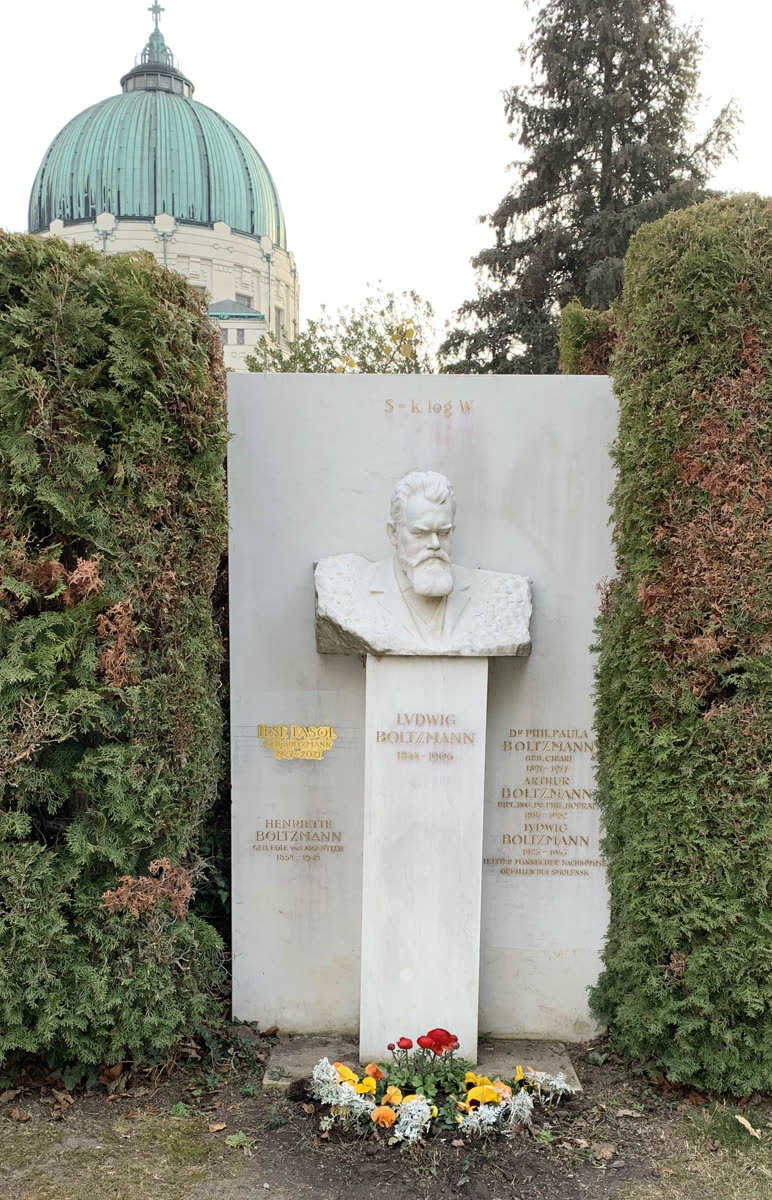
\includegraphics[width=\linewidth]{images/book4/boltzmann-grave.jpg}\par
{\footnotesize La tombe de Boltzmann.}
\end{minipage}
\end{history}

\section{Exercices}

\begin{exercise}[$\star$]\label{exo:b3:partition-functions:1}
Quatre oscillateurs se partagent quatre quanta. Énumérer les
distributions, donner le poids de chacune, et vérifier que leur somme est
égale au nombre de façons de placer quatre quanta \omterm{def:b3:many-electron-atoms:indistinguishable}{indiscernables} dans
quatre oscillateurs, $\binom{7}{3}$. Quelles distributions sont les plus
probables~?
\end{exercise}

\begin{exercise}[$\star$]\label{exo:b3:partition-functions:2}
Deux niveaux non dégénérés sont séparés de \qty{2.5}{kJ/mol}. Calculer le
rapport de leurs \omterm{def:b3:partition-functions:boltzmann}{populations} à \qty{298.15}{K} et à \qty{1000}{K}.
Quelle est la limite à très haute température~?
\end{exercise}

\begin{exercise}[$\star$]\label{exo:b3:partition-functions:3}
% ledger: aw:Ar
Calculer la \omterm{def:b3:partition-functions:thermal-wavelength}{longueur d'onde thermique} d'un atome d'argon à
\qty{298.15}{K} et sa fonction de partition de translation dans un volume
de \qty{1}{dm^3}.
\end{exercise}

\begin{exercise}[$\star$]\label{exo:b3:partition-functions:4}
% ledger: diat:N2.Be, diat:N2.ae, diat:HCl.Be, diat:HCl.ae
Avec $B_0 = \qty{1.990}{cm^{-1}}$ (\ce{N2}) et \qty{10.440}{cm^{-1}}
(\ce{H^{35}Cl}), calculer $\theta_{\mathrm R}$ et la fonction de
partition de rotation de haute température de chaque molécule à
\qty{298.15}{K}.
\end{exercise}

\begin{exercise}[$\star\star$]\label{exo:b3:partition-functions:5}
% ledger: diat:I2.we, diat:I2.wexe, diat:N2.we, diat:N2.wexe
Les nombres d'onde fondamentaux de \ce{I2} et de \ce{N2} valent
\qty{213.27}{cm^{-1}} et
\qty{2329.92}{cm^{-1}}. Calculer $\theta_{\mathrm V}$, $q^{\mathrm V}$ à
\qty{298.15}{K}, et la fraction des molécules qui ne sont pas dans
$v = 0$.
\end{exercise}

\begin{exercise}[$\star\star$]\label{exo:b3:partition-functions:6}
% ledger: diat:NO.split, lev:Cl.2P1_2
Calculer la fonction de partition électronique à \qty{298.15}{K} de
\ce{NO} (deux niveaux doublement dégénérés distants de
\qty{119.73}{cm^{-1}}) et de l'atome de chlore (niveau fondamental
${}^2P_{3/2}$, niveau ${}^2P_{1/2}$ à \qty{882.35}{cm^{-1}}). Quelle
fraction des molécules de \ce{NO} se trouve dans le niveau supérieur~?
Vers quoi tend $q^{\mathrm E}(\ce{NO})$ à haute température~?
\end{exercise}

\begin{exercise}[$\star\star$]\label{exo:b3:partition-functions:7}
À partir de $q^{\mathrm T} = V/\Lambda^3$, établir l'énergie interne et la
capacité thermique à volume constant d'une mole de gaz parfait
monoatomique, et évaluer $U - U(0)$ à
\qty{298.15}{K}.
\end{exercise}

\begin{exercise}[$\star\star$]\label{exo:b3:partition-functions:8}
% ledger: aw:Ar, s0:Ar_g
Utiliser l'équation de Sackur--Tetrode pour calculer l'entropie molaire
standard de l'argon à \qty{298.15}{K}~; comparer à la valeur tabulée
\qty{154.846}{J.K^{-1}.mol^{-1}}. De combien varie-t-elle si l'on divise
la pression par 10~?
\end{exercise}

\begin{exercise}[$\star\star$]\label{exo:b3:partition-functions:9}
% ledger: diat:HCl.Be, diat:HCl.ae
Calculer la contribution de rotation à l'entropie molaire standard de
\ce{H^{35}Cl} à \qty{298.15}{K} ($\theta_{\mathrm R} = \qty{15.02}{K}$).
\end{exercise}

\begin{exercise}[$\star\star\star$]\label{exo:b3:partition-functions:10}
En traitant $J$ comme une variable continue, montrer que le niveau de
rotation le plus peuplé d'une molécule linéaire se situe vers
$J_{\max} = \sqrt{T/2\theta_{\mathrm R}} - \frac12$. L'évaluer pour \ce{HCl}
($\theta_{\mathrm R} = \qty{15.02}{K}$) et \ce{CO} ($\theta_{\mathrm R} = \qty{2.766}{K}$)
à \qty{300}{K}. Pourquoi les deux
branches d'une bande infrarouge sont-elles les plus intenses à quelques
raies du centre~?
\end{exercise}

\begin{exercise}[$\star\star\star$]\label{exo:b3:partition-functions:11}
% ledger: diat:H2.Be, diat:H2.ae
La formule d'Euler--Maclaurin donne $\sum_{J\ge0}f(J) \approx \int_0^\infty f(J)\dd J + \frac12f(0) -
\frac1{12}f'(0)$. L'appliquer à $f(J) = (2J+1)\eu^{-\theta J(J+1)/T}$ et
montrer que $q^{\mathrm R} \approx T/\theta +
\frac13$. Pour quelles températures $T/\theta$ est-il exact à 1\,\% près~?
Est-il acceptable pour \ce{H2}
($B_0 = \qty{59.32}{cm^{-1}}$) à \qty{298.15}{K}~?
\end{exercise}

\begin{exercise}[$\star\star\star$]\label{exo:b3:partition-functions:12}
% ledger: diat:I2.we, diat:I2.wexe
Montrer que l'entropie molaire de vibration tend vers zéro quand
$T \ll \theta_{\mathrm V}$ et vers
$R[1 + \ln(T/\theta_{\mathrm V})]$ quand $T \gg \theta_{\mathrm V}$.
Évaluer à la fois l'expression exacte et cette limite pour \ce{I2}
($\theta_{\mathrm V} = \qty{306.9}{K}$) à \qty{298.15}{K}, et commenter.
\end{exercise}

\section{Problème~: dénombrer l'entropie du diazote}

\begin{problem}[{Problème du week-end --- dénombrer l'entropie du
diazote~: les contributions de translation, de rotation, de vibration et
électronique à son entropie standard, calculées à partir de son spectre
et comparées à la table}]
\label{pb:b3:partition-functions:1}
% ledger: aw:N, diat:N2.Be, diat:N2.ae, diat:N2.we, diat:N2.wexe, s0:N2_g, const:h, const:kB, const:NA, const:c
Le diazote est le principal gaz de l'air. Son entropie molaire standard à
\qty{298.15}{K} est calculée ici à partir de sa masse molaire,
\qty{28.014}{g/mol}, et de ses
constantes spectroscopiques~: $B_e = \qty{1.998241}{cm^{-1}}$, $\alpha_e = \qty{0.017318}{cm^{-1}}$, $\omega_e =
\qty{2358.57}{cm^{-1}}$, $\omega_ex_e = \qty{14.324}{cm^{-1}}$~; son terme
électronique fondamental est ${}^1\Sigma_g^+$.
Pression standard $p^\circ = \qty{1}{bar}$~; $k = \qty{1.380649e-23}{J/K}$, $h = \qty{6.62607015e-34}{J.s}$.

\medskip\noindent\textbf{Partie I --- La translation.}
\begin{enumerate}
  \item Calculer la masse d'une molécule.
  \item Calculer sa \omterm{def:b3:partition-functions:thermal-wavelength}{longueur d'onde thermique} à \qty{298.15}{K}.
  \item Calculer le volume disponible par molécule, $kT/p^\circ$.
  \item En déduire $q^{\mathrm T}/N$, et commenter son ordre de grandeur.
  \item Calculer l'entropie molaire de translation.
  \item De combien varierait-elle sous une pression deux fois plus
        faible~?
\end{enumerate}

\medskip\noindent\textbf{Partie II --- La rotation.}
\begin{enumerate}[resume]
  \item Calculer $B_0$.
  \item Calculer $\theta_{\mathrm R}$.
  \item Donner le \omterm{def:b3:partition-functions:symmetry-number}{nombre de symétrie} et dire ce dont il rend compte.
  \item Calculer $q^{\mathrm R}$ à \qty{298.15}{K}.
  \item La forme de haute température est-elle justifiée~?
  \item Calculer l'entropie molaire de rotation.
  \item En ignorant les poids de spin nucléaire, quel niveau de rotation
        est le plus peuplé~?
\end{enumerate}

\medskip\noindent\textbf{Partie III --- Vibration et états électroniques.}
\begin{enumerate}[resume]
  \item Calculer le quantum de vibration $G(1) - G(0)$.
  \item Calculer $\theta_{\mathrm V}$.
  \item Calculer $q^{\mathrm V}$ à \qty{298.15}{K}.
  \item Quelle fraction des molécules se trouve dans $v = 1$~?
  \item Calculer l'entropie molaire de vibration.
  \item Quelle est la contribution électronique~? Pourquoi peut-on
        ignorer les états électroniques excités~?
\end{enumerate}

\medskip\noindent\textbf{Partie IV --- Somme et comparaison.}
\begin{enumerate}[resume]
  \item Additionner les contributions.
  \item Comparer à la valeur tabulée, \qty{191.609}{J.K^{-1}.mol^{-1}}.
  \item Sur quelles mesures repose la valeur calorimétrique d'une
        table~?
  \item Pourquoi les tables peuvent-elles laisser de côté le spin
        nucléaire~?
  \item Énoncer le résultat~: l'entropie molaire standard du diazote à
        \qty{298.15}{K} calculée à partir de ses constantes
        spectroscopiques.
\end{enumerate}
\end{problem}
